\section{IDLE}

	IDLE is Python's editor, used to edit and run Python programs on your Pi. You can find it under \texttt{Programming > IDLE} from the Raspberry Pi logo in the top left of your screen. There may be more than 1 version of IDLE, as Raspbian comes with both Python 2 and Python 3 installed. Python 3 is the preferred choice (although this booklet will work with Python 2 as well), as it has some improvements over Python 2.

	IDLE opens into it's shell by default, allowing you to enter code and have it run immediately without having to create and save any files. Note that this shell doesn't save your code for you, so make sure you save any code you want to keep!

	\begin{center}
		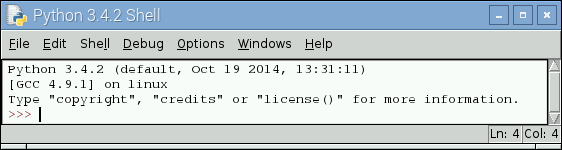
\includegraphics[width=120mm]{McrRaspJam/014_Python/1_idle/screenshot}
	\end{center}

	Try typing the following code into the shell and hitting enter.

	\lstinputlisting[style=Python, numbers=none]{McrRaspJam/014_Python/1_idle/hello_world.py}

	You should get the following output after hitting enter.

	\begin{lstlisting}[style=Terminal, numbers=none]
Hello, World!
	\end{lstlisting}

	Now, compare that to the equivalent Java program:

	\lstinputlisting[style=Java, numbers=none]{McrRaspJam/014_Python/1_idle/HelloWorld.java}

	As opposed to Java, Python is a simple language in which a lot of functionality is implicit and not explicit. There is no need for \texttt{System.out.println} or even the \texttt{main} function, as Python provides them for you.

	\begin{aside}[Execution]
		Code in Python is executed from top to bottom in every file, meaning no \texttt{main} method is required. Simply placing the code in a file is enough for it to run!
	\end{aside}
